\documentclass[10pt]{article}
\usepackage[utf8]{inputenc}
\usepackage{mathtools}
\usepackage{graphicx}
\usepackage{array}
\usepackage[margin=0.5in]{geometry}
\usepackage{listings}
\usepackage{color}

\definecolor{mygreen}{rgb}{0,0.6,0}
\definecolor{mygray}{rgb}{0.5,0.5,0.5}
\definecolor{mymauve}{rgb}{0.58,0,0.82}

\lstset{ %
  backgroundcolor=\color{white},   % choose the background color; you must add \usepackage{color} or \usepackage{xcolor}; should come as last argument
  basicstyle=\footnotesize,        % the size of the fonts that are used for the code
  breakatwhitespace=false,         % sets if automatic breaks should only happen at whitespace
  breaklines=true,                 % sets automatic line breaking
  captionpos=b,                    % sets the caption-position to bottom
  commentstyle=\color{mygreen},    % comment style
  deletekeywords={...},            % if you want to delete keywords from the given language
  escapeinside={\%*}{*)},          % if you want to add LaTeX within your code
  extendedchars=true,              % lets you use non-ASCII characters; for 8-bits encodings only, does not work with UTF-8
  frame=single,	                   % adds a frame around the code
  keepspaces=true,                 % keeps spaces in text, useful for keeping indentation of code (possibly needs columns=flexible)
  keywordstyle=\color{blue},       % keyword style
  language=Octave,                 % the language of the code
  morekeywords={*,...},            % if you want to add more keywords to the set
  numbers=left,                    % where to put the line-numbers; possible values are (none, left, right)
  numbersep=5pt,                   % how far the line-numbers are from the code
  numberstyle=\tiny\color{mygray}, % the style that is used for the line-numbers
  rulecolor=\color{black},         % if not set, the frame-color may be changed on line-breaks within not-black text (e.g. comments (green here))
  showspaces=false,                % show spaces everywhere adding particular underscores; it overrides 'showstringspaces'
  showstringspaces=false,          % underline spaces within strings only
  showtabs=false,                  % show tabs within strings adding particular underscores
  stepnumber=2,                    % the step between two line-numbers. If it's 1, each line will be numbered
  stringstyle=\color{mymauve},     % string literal style
  tabsize=2,	                   % sets default tabsize to 2 spaces
  title=\lstname                   % show the filename of files included with \lstinputlisting; also try caption instead of title
}
\renewcommand{\arraystretch}{1.5}
\setcounter{secnumdepth}{0}
\author{Kevin Mambu}
\date{\today}

\title{M1 SESI 2017-2018\\Architecture Multi-Processeurs\\TP2 : Déploiement de
code sur processeur programmable}

\begin{document}
\maketitle

\section{Énoncé du TP}
Objectif : exécution d'une application logicielle en C sur une architecture
comportant un processeur MIPS32.
\begin{itemize}
  \item Cross-compilateur gcc-mipsel
  \item Chargement du fichier binaire
\end{itemize}

\subsection{Propriétés de l'Architecture}
\begin{itemize}
  \item Processeur MIPS32 Pipeliné (5 étages)
  \item Cache d'instruction :
  \begin{itemize}
    \item Direct Mapping
    \item \#ligne = 16 octets
    \item \#cache = 1 Ko
    \item \#lignes = 64 lignes
  \end{itemize}
  \item Cache de données :
  \begin{itemize}
    \item Mêmes spécifications que le cache d'instruction
    \item Politique Write-Through
  \end{itemize}
  \item Le contrôleur déclenche une transaction sur le PIBUS dnas les cas suivants :
  \begin{itemize}
    \item miss instruction : demande d'instruction non-chargée\\
    \begin{center}
      ${MISS\_INST_{\#cy}}=\underbrace{1}_{detect MISS}+\underbrace{4*1}_{Rafale}+\underbrace{1}_{dernier ACK}$
    \end{center}
    \item miss data : ${MISS\_DATA_{\#cy}} = {MISS\_INST_{\#cy}}$
    \item read uncached : lecture de donnée non-cachable (dépend du segment lu)
  \end{itemize}
\end{itemize}

\subsection{Le GIET}
Le Gestionnaire d'Interruption, d'Exception et de Trappes (GIET) est le système
d'exploitation utilisé sur cette architecture lors de ce TP.\\
S'il ne fournit pas le support de mémoire virtuelle et de création dynamique
de tâches, il support les architectures multi-processeurs, permettant quand même
l'exécution concurrente de tâches créées statiquement.\\
\begin{itemize}
  \item sys\_hander.c : gestionnaire d'appels systèmes
  \item exc\_handler.c: gestionnaire d'exceptions
  \item irq\_handler.c: gestionnaire d'interruptions
  \item ctx\_handler.c: context switcher (mutiplexage temporel)
  \item drivers.c : méthodes d'accès aux périphériques
\end{itemize}

\subsection{Boot Record, Bootloader et {\it Soclib::Loader}}
Le Bootloader est un programme stocké en ROM, lancé au démarrage et chargé entre
autres des tâches suivantes :
\begin{itemize}
  \item vérification du bon fonctionnement du matériels
  \item tests sur le système
  \item populer la mémoire vive du système d'exploitation (chargement DD $\rightarrow$ RAM)
\end{itemize}

Parce que le rapport temporel entre la machine simulée et la machine simulante
est élevée (1MHz contre 1GHz), SoCLib fournit un objet de programmation permettant
de pré-charger par la machine simulante la mémoire vive avant simulation, pour
faire abstraction du temps de chargement : il s'agit de la classe {\it SoCLib::Loader}.\\
Le loader peut charger différents types de fichiers, dont deux en particulier :
\begin{itemize}
  \item les Binary Large OBject (blobs), des paquets binaires non-structurés.
  \item les ficheiers binaires générés par GCC (.bin, .elf) avec des métadonnées
  en entête.
\end{itemize}

\subsection{Memory Map}
\begin{tabular}{|c|c|c|c|}
  \hline
  segment & adresse & taille & composant \\ \hline
  seg\_tty & 0x9000 0000 & 16 Ko & PIBUS\_MULTI\_TTY \\ \hline
  seg\_reset & 0xBFC0 0000 & 4 Ko & ROM \\ \hline
  seg\_kcode & 0x8000 0000 & 16 Ko & RAM \\ \hline
  seg\_kunc & 0x8100 0000 & 4 Ko & RAM \\ \hline
  seg\_kdata & 0x8200 0000 & 64 Ko & RAM \\ \hline
  seg\_code & 0x0040 0000 & 16 Ko & RAM \\ \hline
  seg\_data & 0x0100 0000 & 16 Ko & RAM \\ \hline
  seg\_stack & 0x0200 0000 & 16 Ko & RAM \\ \hline
\end{tabular}

\subsection{Répertoire soft/Dépendances}
\lstinputlisting[]{filetree.txt}

\subsection{MIPS - Table des Registres}
\begin{center}
  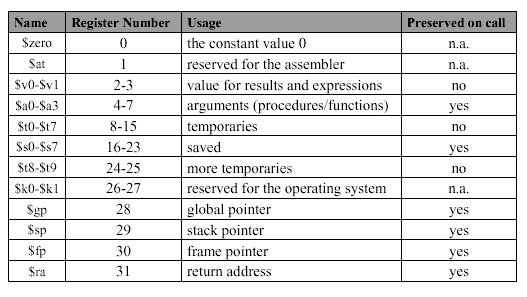
\includegraphics[width=11cm]{mips-table.jpg}\\
\end{center}
\newpage

\section{Question C1}
\lstinputlisting[language=C++,firstline=75,lastline=81]{tp2_top.cpp}

\section{Question C2}
{\it seg\_reset} contient le code {\bf boot} et doit être chargé de manière
systématique à chaque démarrage de machine. De ce fait, il doit être stocké dans
une mémoire statique et non-modifiable (Read-Only Memory), alors que les segments
({\it kcode, kdata}, etc) sont dans une mémoire volatile et potentiellement
modifiable (Random Access Memory).

\section{Question C3}
Le segment {\it seg\_tty} ne doit pas être cachable car les valeurs de ses registres
évoluent indépendamment des composants maîtres qui veulent y accéder.

\section{Question C4}
Les segments protégés sont ({\it seg\_reset, seg\_kcode, seg\_kunc, seg\_kdata, seg\_tty}).\\
Ces segments sont délimités des segments utilisateurs par leur adressage:
\begin{itemize}
  \item L'espace utilisateur correspond à la moitié basse
    $[0x00000000,0x7FFFFFFF]$ de l'espace d'adressage.
  \item L'espace privilégié correspond à la moitié haute
    $[0x80000000,0xFFFFFFFF]$ de l'espace d'adressage.
\end{itemize}

\section{Question D1}
Lors d'un appel système, un programme utilisateur doit fournir au systéme
d'exploitation le numéro de l'appel système ainsi que ses arguments (4 max.).\\
Pour transmettre ces informations, la méthode {\it sys\_call} charge ses paramétres
en registres internes du processeur avant de faire un appel système.

\section{Question D2}
{\it \_cause\_vector} contient des valeurs, chaqu'une associée à un cas d'entrée
au GIET possible. Il est initialisé dans le fichier {\it exc\_handler.c}.\\
{\it \_syscall\_vector} contient les points d'entrées vers les adresses de chaque
appel système. On pourrait dire qu'il s'agit d'une table de hash. Il est initialisé
dans le fichier {\it sys\_handler.c}.

\section{Question D3/D4}
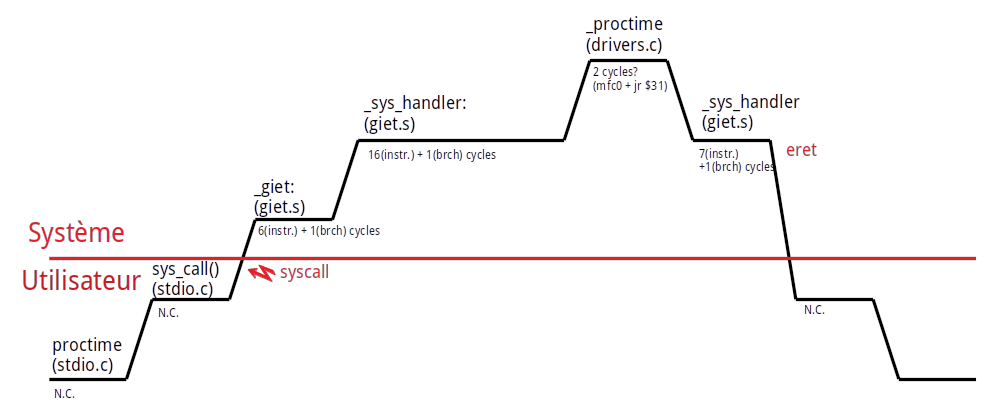
\includegraphics[width=18cm]{chrono.png}\\
Déterminer la durée d'exécution de {\it proctime()} est compliqué, vu que les temps
en cycles de {\it sys\_call()} et {\it proctime()} dépendent de la compilation.

\section{Question E1}
Le code de {\bf boot} doit nécéssairement s'exécuter en mode superviseur pour
trois raisons :
\begin{itemize}
  \item Le segment qui lui est affilié par convention se trouve dans l'espace
  privilégié.
  \item Il doit charger en ménoire le système d'exploitation, or les segments
  affiliés par convention à l'OS se trouvent dans l'espace privilégié, le code
  de boot à donc besoin de privilèges particuliers pour pouvoir charger des
  données dans cette zone.
\end{itemize}

\section{Question E2}
Par convention le segment de code de l'application utilisateur, {\bf code},
commence à l'adresse 0x0040 0000. C'est à cette adresse que le code de {\bf boot}
va systématiquement se brancher après avoir populé la RAM.

\section{Question E3}
Si les adresses de bases de segments spécifiées par le matériel sont différentes
de celles spécifiées dans le logiciel utilisateur, ce dernier a de fortes chances
de se faire tuer pour Erreur de Segmentation, en tentant d'acceder à une zone de
l'espace d'adressage non-repertoriée.

\section{Question E4}
{\it reset.o} est chargé au segment {\bf boot}. {\it giet.o} au segment {\bf kcode}.

\newpage

\section{Question E5}
{\it seg\_reset} :
\begin{itemize}
  \item première instr. à 0xBFC0 0000
  \item dernière instr. à 0xBFC0 0024
  \item 10 instructions, 40 octets
\end{itemize}
{\it seg\_kcode} :
\begin{itemize}
  \item première instr. à 0x8000 0000
  \item dernière instr. à 0x8000 2208
  \item 2179 instructions, 8716 octets
\end{itemize}

\section{Question E6}
\lstinputlisting[language=C]{soft/main.c}

\section{Question E7}
L'appel {\it tty\_getc()} fonctionne comme suit : elle appele en boucle la fonction
système {\it \_tty\_read()} et teste sa valeur de retour. Si cette dernière est
différente de 0 alors la boucle est intérrompue.\\
Il faut mettre cette attente active dans {\it tty\_getc()} et non {\it \_tty\_read()}
parce que :
\begin{enumerate}
  \item L'utilisateur fait appel à ce service donc ça doit être lui qui supporte
  les potentielles charges de temporisation, attendant la réponse à sa requête.
  \item On ne peut pas se permettre un mécanisme de bloquage en mode système
  en lieu à cause de l'utilisateur. Ce dernier ne doit pas pouvoir entraver le
  bon fonctionnement de l'OS.
\end{enumerate}

\section{Question E8}
{\it seg\_code} :
\begin{itemize}
  \item première instr. à 0x0040 0000
  \item dernière instr. à 0x0040 013C
  \item 1219 instructions, 4876 octets
\end{itemize}

\newpage{}
\section{Question E9}
\lstinputlisting[language=bash]{soft/Makefile}
\newpage{}

\section{Question F1}
La première transaction sur le bus est à la suite d'un {\it miss instruction},
le miss est compulsif car le cache est encore vide à ce moment. Le processeur va
demander les instructions situées en ROM.\\
Cela arrive dès le cycle 0 :
\lstinputlisting[firstline=60,lastline=81]{trace.txt}
La première instruction du boot est :
\lstinputlisting[firstline=8,lastline=8]{sys.bin.txt}
Cela se fait au cycle 10 :
\lstinputlisting[firstline=280,lastline=301]{trace.txt}
\newpage
La deuxième transaction s'effectue au cycle 14 :
\lstinputlisting[firstline=368,lastline=389]{trace.txt}
Cela correspond à cette instruction (note : après le 3e cours on sait maintenant
qu'il s'agit d'une ecriture externe) :
\lstinputlisting[firstline=12,lastline=12]{sys.bin.txt}

\newpage

\section{Question F2}
La première instruction du main est :
\lstinputlisting[firstline=1282,lastline=1283]{app.bin.txt}
Cela se fait au cycle 57 :
\lstinputlisting[firstline=1314,lastline=1335]{trace.txt}

\section{Question F3}
La première transaction corresondant à la lecture de la chaine de caractères "Hello
World!" se fait au cycle 32 :
\lstinputlisting[firstline=764,lastline=785]{trace.txt}
\newpage
\section{Question F4}
L'appel de tty\_puts() entraine un appel à la commande du pilote du TTY \_tty\_write() :
\lstinputlisting[firstline=339,lastline=339]{sys.bin.txt}
Dans \_tty\_write(), l'instruction d'ecriture d'un caractère est :
\lstinputlisting[firstline=400,lastline=400]{sys.bin.txt}
Je n'ai pas réussi à retrouver cette instruction dans la trace.

\end{document}
